% $Id: template.tex 11 2007-04-03 22:25:53Z jpeltier $

\documentclass{vgtc}                          % final (conference style)
%\documentclass[review]{vgtc}                 % review
%\documentclass[widereview]{vgtc}             % wide-spaced review
%\documentclass[preprint]{vgtc}               % preprint
%\documentclass[electronic]{vgtc}             % electronic version

%% Uncomment one of the lines above depending on where your paper is
%% in the conference process. ``review'' and ``widereview'' are for review
%% submission, ``preprint'' is for pre-publication, and the final version
%% doesn't use a specific qualifier. Further, ``electronic'' includes
%% hyperreferences for more convenient online viewing.

%% Please use one of the ``review'' options in combination with the
%% assigned online id (see below) ONLY if your paper uses a double blind
%% review process. Some conferences, like IEEE Vis and InfoVis, have NOT
%% in the past.

%% Figures should be in CMYK or Grey scale format, otherwise, colour 
%% shifting may occur during the printing process.

%% These few lines make a distinction between latex and pdflatex calls and they
%% bring in essential packages for graphics and font handling.
%% Note that due to the \DeclareGraphicsExtensions{} call it is no longer necessary
%% to provide the the path and extension of a graphics file:
%% \includegraphics{diamondrule} is completely sufficient.
%%
\ifpdf%                                % if we use pdflatex
  \pdfoutput=1\relax                   % create PDFs from pdfLaTeX
  \pdfcompresslevel=9                  % PDF Compression
  \pdfoptionpdfminorversion=7          % create PDF 1.7
  \ExecuteOptions{pdftex}
  \usepackage{graphicx}                % allow us to embed graphics files
  \DeclareGraphicsExtensions{.pdf,.png,.jpg,.jpeg} % for pdflatex we expect .pdf, .png, or .jpg files
\else%                                 % else we use pure latex
  \ExecuteOptions{dvips}
  \usepackage{graphicx}                % allow us to embed graphics files
  \DeclareGraphicsExtensions{.eps}     % for pure latex we expect eps files
\fi%

%% it is recomended to use ``\autoref{sec:bla}'' instead of ``Fig.~\ref{sec:bla}''
\graphicspath{{figures/}{pictures/}{images/}{./}} % where to search for the images

\usepackage{microtype}                 % use micro-typography (slightly more compact, better to read)
\PassOptionsToPackage{warn}{textcomp}  % to address font issues with \textrightarrow
\usepackage{textcomp}                  % use better special symbols
\usepackage{mathptmx}                  % use matching math font
\usepackage{times}                     % we use Times as the main font
\renewcommand*\ttdefault{txtt}         % a nicer typewriter font
\usepackage{cite}                      % needed to automatically sort the references
\usepackage{tabu}                      % only used for the table example
\usepackage{booktabs}                  % only used for the table example
%% We encourage the use of mathptmx for consistent usage of times font
%% throughout the proceedings. However, if you encounter conflicts
%% with other math-related packages, you may want to disable it.


%% If you are submitting a paper to a conference for review with a double
%% blind reviewing process, please replace the value ``0'' below with your
%% OnlineID. Otherwise, you may safely leave it at ``0''.
\onlineid{0}

%% declare the category of your paper, only shown in review mode
\vgtccategory{Research}

%% allow for this line if you want the electronic option to work properly
\vgtcinsertpkg

%% In preprint mode you may define your own headline. If not, the default IEEE copyright message will appear in preprint mode.
%\preprinttext{To appear in an IEEE VGTC sponsored conference.}

%% This adds a link to the version of the paper on IEEEXplore
%% Uncomment this line when you produce a preprint version of the article 
%% after the article receives a DOI for the paper from IEEE
%\ieeedoi{xx.xxxx/TVCG.201x.xxxxxxx}


%% Paper title.

\title{Web Voyager: Lightweight Exploration Of Semi-Structured Website Data}

%% This is how authors are specified in the conference style

%% Author and Affiliation (multiple authors with single affiliations).
\author{Kapaya Katongo\thanks{e-mail: kkatongo@mit.edu}
\and Geoffrey Litt\thanks{e-mail: glitt@mit.edu}
\and Daniel Jackson\thanks{e-mail: dnj@csail.mit.edu}}
\affiliation{\scriptsize MIT CSAIL}

%% Abstract section.
\abstract{
 Websites are awash with semi-structured data that is ripe for exploration but there are two significant barriers to this: accessing the data and visualizing it. Accessing the data requires web scraping because the data is often not available in a portable format such as JSON or CSV or is only available behind an API which requires programming expertise to use. Visualizing the data requires knowledge of visualization specification formats or languages.

 In this paper, we present an interaction model for lightweight exploration of semi-structured website data that does not require knowledge of web scraping or data visualization formats and languages. Our key idea is to combine web scraping via programming-by-demonstration with visualization recommendation: users scrape data from a website via mouse clicks and get visualization recommendations based on the scraped data. Unlike existing solutions, our web scraping approach supports accessing a wide variety of semi-structured website data and our visualization approach is neither limited to predefined visualizations nor does it require knowledge of data visualization.

 To illustrate the proposed model, we have implemented a Chrome browser extension called Web Voyager. Through case studies, we show how our model can be used to explore data on real-world websites in order to characterize the capabilities and limitations of the approach.
} % end of abstract

%% ACM Computing Classification System (CCS). 
%% See <http://www.acm.org/about/class> for details.
%% We recommend the 2012 system <http://www.acm.org/about/class/class/2012>
%% For the 2012 system use the ``\CCScatTwelve'' which command takes four arguments.
%% The 1998 system <http://www.acm.org/about/class/class/2012> is still possible
%% For the 1998 system use the ``\CCScat'' which command takes four arguments.
%% In both cases the last two arguments (1998) or last three (2012) can be empty.

\CCScatlist{
  \CCScatTwelve{Human-centered computing}{Visu\-al\-iza\-tion}{Visu\-al\-iza\-tion systems and tools};
}

%% Copyright space is enabled by default as required by guidelines.
%% It is disabled by the 'review' option or via the following command:
% \nocopyrightspace

%%%%%%%%%%%%%%%%%%%%%%%%%%%%%%%%%%%%%%%%%%%%%%%%%%%%%%%%%%%%%%%%
%%%%%%%%%%%%%%%%%%%%%% START OF THE PAPER %%%%%%%%%%%%%%%%%%%%%%
%%%%%%%%%%%%%%%%%%%%%%%%%%%%%%%%%%%%%%%%%%%%%%%%%%%%%%%%%%%%%%%%%

\begin{document}

%% The ``\maketitle'' command must be the first command after the
%% ``\begin{document}'' command. It prepares and prints the title block.

%% the only exception to this rule is the \firstsection command
\firstsection{Introduction}
\label{introduction}

\maketitle

%% \section{Introduction} %for journal use above \firstsection{..} instead
Many websites provide valuable semi-structured data that users would like to process and visualize. This data ranges from job postings on websites like LinkedIn to user reviews on websites like Yelp. To explore data through visualization, it must be in a format suitable for computation. Most website data is either not available in a portable format (such as JSON or CSV) or is only available via an Application Programming Interface (API) which requires programming expertise to use. Even with the data in hand, visualizing it requires knowledge of data visualization formats and languages. 

Prior research has resulted in tools like Vispedia \cite{chan2008}, Reform \cite{toomim2009} and DS.js \cite{zhang2017} which have developed solutions to overcome some of these barriers. Vispedia automatically accesses website data via web scraping and allows users to visualize it using a predefined list of visualizations, but it only works on Wikipedia. Reform allows users to scrape a site via programming-by-demonstration (PBD) and then feed it into a predefined visualization widget created by a programmer. While the visualization widgets are not restricted to any given website, they require the exact data prescribed by their authors. This means that in order to visualize data on a website, a programmer must have created a visualization widget that accepts that type of data. DS.js comes closest to breaking down the two barriers. It automatically accesses website data via web scraping and provides a programming environment to analyze and visualize the scraped data. However, only website data in HTML table elements can be accessed, which does not cover the wide variety of semi-structured data available on many websites. Furthermore, users require knowledge of programming and data visualization in order to use the provided programming environment to explore the data.

In this paper, we present an interaction model for lightweight exploration of semi-structured website data right in the context of the website. Our key idea is to combine web scraping via PBD with visualization recommendation: users scrape data from a website via mouse clicks and get visualization recommendations based on the scraped data. No knowledge of web scraping or data visualization specification formats and languages is required. Unlike existing solutions, our web scraping approach supports accessing a wide variety of semi-structured website data and our visualization approach is neither limited to predefined visualizations nor does it require knowledge of data visualization.

\begin{figure*}
  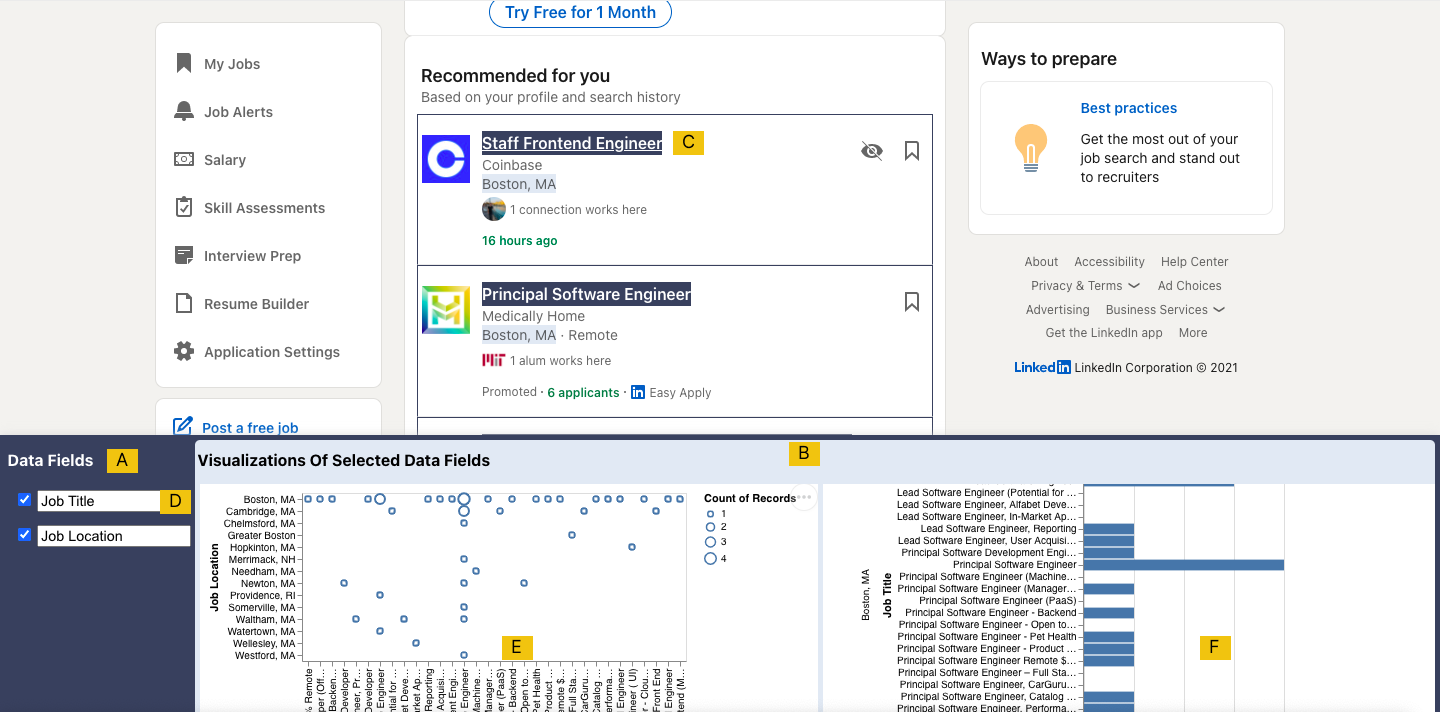
\includegraphics[width=\textwidth]{figures/example}
  \caption{\label{fig:example}An overview of exploring job data on LinkedIn using Web Voyager. A) Data field section, B) Visualization section, C) Scraped job title values, D) Job title data field input and checkbox, E) First visualization recommendation based on job title and job location, F) Second visualization recommendation based on job title and job location}
  \label{fig:example}
\end{figure*}

To illustrate this approach, we implemented a Chrome browser extension called Web Voyager. Web Voyager combines the PBD web scraping techniques we developed for Wildcard \cite{litt2020} to access website data with CompassQL \cite{wongsuphasawat2016}, the query language for visualization recommendation that powers Voyager 2 \cite{wongsuphasawat2017} (the inspiration for our tool’s name). Our contributions are as follows:

\begin{itemize}
 \item An interaction model for lightweight exploration of semi-structured website data via PBD web scraping and visualization recommendation, and
 \item An implementation of the proposed interaction model via a Chrome browser extension.
\end{itemize}

Section \ref{demo} describes a concrete scenario that shows how our model can be used to explore data on a real world website. In Section \ref{implementation}, we outline the implementation of the web scraping approach and our use of CompassQL to recommend visualizations based on the scraped data. To characterize the capabilities and limitations of our model, we present a suite of case studies on real world websites in Section \ref{evaluation}]. In Section \ref{related-work}, we relate our approach to existing work in PDB web scraping and data visualization. Finally, Section \ref{conclusion} discusses opportunities for future work such as giving users more control over the visualization process.

\section{Example Scenario} \label{demo}

This section describes an example scenario, illustrated in Figure \ref{fig:example}, of exploring website data with Web Voyager.
Jen is looking to change jobs and wants to explore a list of job postings on LinkedIn. She is curious about the jobs available, and
wonders whether there are any trends in job title or job location but unfortunately LinkedIn does not provide access to the data outside
of the website. Even if it did, Jen does not have any experience with data visualization formats or languages and her curiosity is not enough
motivation to learn them. Using Web Voyager,Jen can explore the data in the context of the website with a few simple clicks.

She starts out by initiating Web Voyager through the browser context menu. This renders a panel with two sections: one for the data fields
that will represent the data that will be scraped (Figure \ref{fig:example} A) and one for the visualization recommendations (Figure \ref{fig:example} B).
As she hovers over one of the job title values, Web Voyager highlights the job titles across all the jobs which gives her feedback about what values will
be scraped (Figure \ref{fig:example} C). She clicks on the value to scrape all the job titles and Web Voyager adds a checkbox-activated field with the default
label \emph{A} to the data section. Because this is the first field to be scraped, it is automatically checked and results in the recommendation of a visualization
based on the job title data. The recommendation is a univariate visualization with job titles on the y-axis and a count of each job title in the data on the x-axis.
With this, Jen is able to easily see that the most common job title is "Principal Software Engineer."

Jen proceeds to scrape the job location values, which adds a second field (\emph{B}) to the data section whose checkbox is unchecked. To keep track of which
field corresponds to which data values, Jen clicks into the job title data field input, which shows her the corresponding values on the website by highlighting
them, and changes \emph{A} to \emph{Job Title}. This automatically re-renders the visualization to update the y-axis label from \emph{A} to \emph{Job Title}
(Figure \ref{fig:example} D). She likewise changes \emph{B} to \emph{Job Location}, and checks its checkbox. This results in the recommendation of two data
visualizations based on both the job title and job location data. The first visualization (Figure \ref{fig:example} E) has job locations on the y-axis and
job titles on the x-axis, with points sized by the number of jobs at a given location with a given title used as marks. The second visualization
(Figure \ref{fig:example} F) shows a small-multiples bar chart with the count of jobs of each title in a given city. Jen continues to scrape data
values and use the data field checkboxes to determine what visualizations will be recommended based on the data corresponding to checked data fields. 

Using Web Voyager, Jen was able to explore the job data using a few simple clicks without any knowledge of web scraping or data visualization.
In Section \ref{evaluation}, we present a suite of case studies that show more real-world websites whose semi-structured data can be explored
using our interaction model.

\section{Implementation} \label{implementation}

This section outlines the implementation of our web scraping and visualization recommendation approaches. The web scraping approach is based on work we did for end-user web scraping in Wildcard \cite{litt2020} and the visualization recommendation uses CompassQL \cite{wongsuphasawat2016}, the query language for visualization recommendation that powers Voyager 2 \cite{wongsuphasawat2017}.

\subsection{Web Scraping}

When users demonstrate a value to scrape, Web Voyager must synthesize a program that reflects the user’s general intent. This is an instance of the wrapper induction \cite{kushmerick2000} problem of synthesizing a web data extraction query from examples. In the next two sections, we describe the two stages involved in this process.

\subsubsection{Determing Row Elements}

Given a DOM element \(v\) representing a value to scrape, we must find a
set of a set of \emph{row elements} that represent the rows of the
containing data table. We could naively assume that \(parent(v)\) is the
row containing \(v\), but often \(v\) is deeply nested inside its
containing row; we must determine which ancestor of \(v\) is likely to
be the row.

Intuitively, we solve this problem by assuming that all rows share some
similar internal structure. In particular, we expect most rows to
contain a value for the demonstrated column. (If there were no missing
data, we'd expect \emph{all} rows to contain data for this column.)

Formally: assume a function \(select(el, s)\) which runs a CSS selector
that returns the set of elements matching \(s\) within \(el\). We
generate a set of plausible candidates \(P\), consisting of pairs of a
row element and a CSS selector:

\(P = \{ (r, s) \mid r \in ancestors(v) \land select(r, s) = \{v\} \}\)

For each candidate \((r, s) \in P\), we compute a weight function \(w\),
which is based on the number of siblings of \(r\) that have ``similar
structure,'' defined by checking whether running \(s\) within the
sibling also returns a unique element.

\(w(r, s) = |\{ r' \mid r' \in siblings(r) \land |select(r', s) | = 1 \}|\)

We then choose the candidate with the highest weight. In case of ties,
the candidate closer to \(v\) in the tree (i.e., lower in the tree)
wins. Given a winning candidate \((r, s)\), the full set of row elements
is \(\{r\} \cup siblings(r)\).

\begin{figure*}
  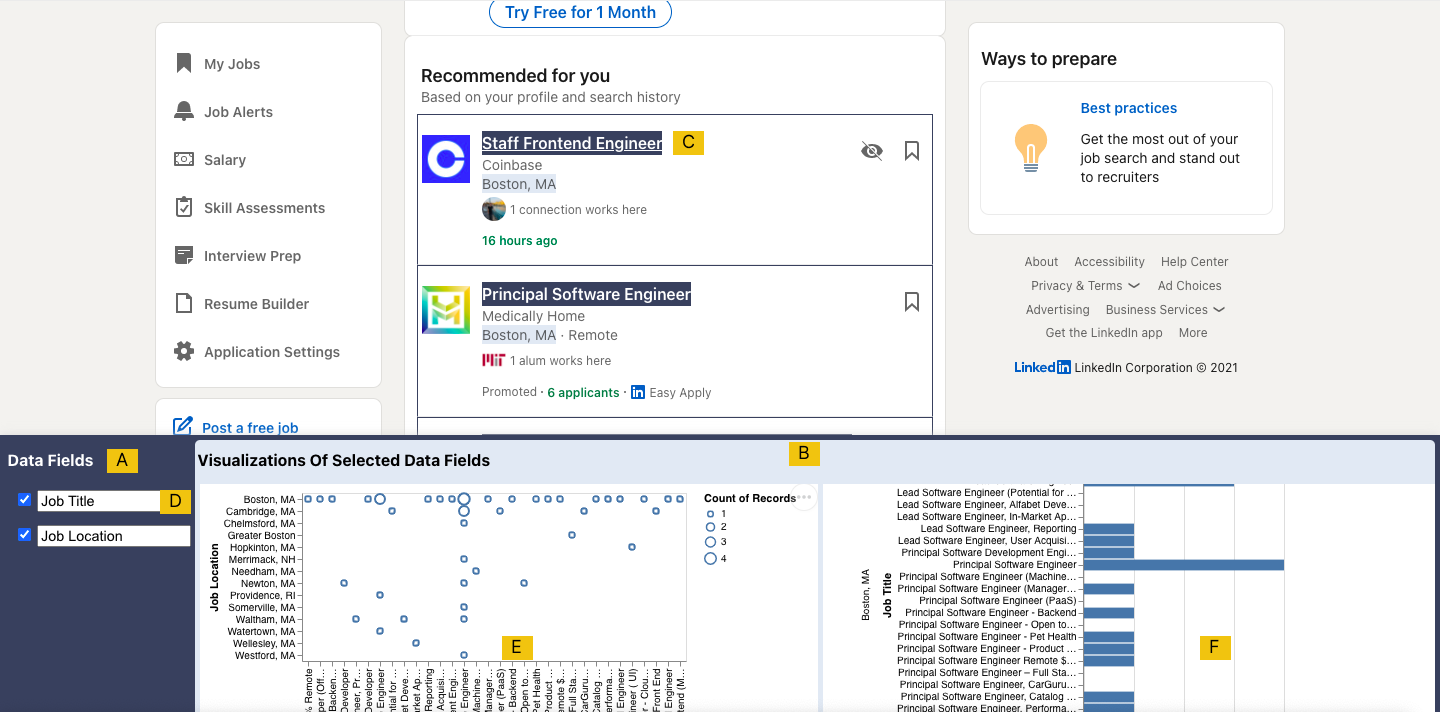
\includegraphics[width=\textwidth]{figures/example}
  \caption{\label{fig:example}An overview of exploring job data on LinkedIn using Web Voyager. A) Data field section, B) Visualization section, C) Scraped job title values, D) Job title data field input and checkbox, E) First visualization recommendation based on job title and job location, F) Second visualization recommendation based on job title and job location}
  \label{fig:example}
\end{figure*}

\subsubsection{Synthesizing CSS Selectors For Column
Values}

Once we have determined the row elements, next we must choose a CSS
selector that will be used to identify the demonstrated value within its
row.

Given a demonstrated value \(v\) within a row element \(r\), we generate
two kinds of plausible selectors:

\begin{itemize}
\item
  selectors using CSS classes, which are manual annotations on DOM
  elements added by the website's programmers, typically for styling
  purposes (e.g.~"item\_\_price")
\item
  selectors using positional indexes within the tree, using the
  \texttt{nth-child} CSS selector (e.g.~\texttt{nth-child(2)},
  representing the second child of an element)
\end{itemize}

The minimum criteria for a plausible selector \(s\) is that it uniquely
identifies the value within the row: \(select(r, s) = \{v\}\). But there
may be many plausible selectors, so we must pick a best one.

We first prioritize selectors using classes, because they tend to be
more robust to changes on the website and are more readable. A single
selector can combine multiple classes, but we prefer using fewer classes
when possible. If no plausible class-based selector can be generated
(for example, if the relevant elements don't have any classes to query),
we fall back to using a positional index selector. This kind of selector
can always be generated regardless of the contents of the page, but
tends to be less accurate and robust.

\subsection{Visualization Recommendation}

Web Voyager's visualization recommendation uses CompassQL, the query
language for visualization recommendation that powers Voyager 2. At a
high level, Web Voyager takes the selected data fields (determined by
the checkboxes) and the full set of scraped data and uses them to define
a CompassQL query.

Once executed, the query results in a ranked list of Vega-lite
\cite{satyanarayan2017} visualization specifications which are used to
render visualizations using Vega-lite. CompassQL provides three key
features that enable this visualization recommendation based on a list
of selected data fields and the complete set of data. The sections below
describe each of the three features.

\subsubsection{Specification}

CompassQL queries are defined using Vega-lite's visualization grammar
with an enumeration token to indicate which properties should be
enumerated to generate multiple visualization specifications. Web
Voyager creates a query with the values of the \texttt{mark} and
\texttt{channel} properties set to an enumeration token (\texttt{?}).
This instructs CompassQL to generate visualization specifications based
on the enumeration of marks (\texttt{bar}, \texttt{point},
\texttt{circle}, \texttt{line} etc) and channels (\texttt{x},
\texttt{y}, \texttt{size}, \texttt{color} etc).

\subsubsection{Choosing and Ordering}

CompassQL queries can define properties that determine how to choose the
top visualization specification (\texttt{chooseBy}) or how to order
visualization specifications by a ranking criteria (\texttt{orderBy}).
Web Voyager creates queries with the value of \texttt{orderBy} set to
\texttt{effectiveness}.

\subsubsection{Grouping and Nesting}

CompassQL queries can define \texttt{groupBy} and \texttt{nest}
properties to reduce redundancy in the list of resulting visualization
specifications. The redundancy stems from the fact that there may be
many visualizations with similar encodings or data. Web Voyager creates
queries with \texttt{groupBy} and \texttt{nest} that group and nest
visualization specifications by properties such as \texttt{channel} and
\texttt{field}.

\section{Evaluation} \label{evaluation}

In this section, we characterize the capabilities of our interaction
model through a suite of case studies on real world websites. Then, we
outline the limitations of our web scraping and data visualization
approaches.

\subsection{Case Studies}

We used Web Voyager to explore data on a collection of real world
websites that we list in Table 1. The websites were chosen to showcase
the variety of supported semi-structured data available on websites.

\subsection{Limitations}

In this section, we outline the limitations of our web scraping and data
visualization approaches using real world websites as references.

\subsubsection{Web Scraping}

Web Voyager' web scraping approach is most effective on websites whose
data is presented in its entirety and as a collection of similarly-structured HTML elements.
Certain websites, however, have designs that make it difficult to scrape
data:

\emph{Heterogeneous Row Elements}. Websites like HackerNews break their content into rows, but the rows do
not have a consistent layout, and contain different types of child
elements. Because Web Voyager only chooses a single row selector, when
scraping by demonstration, it will only select one of the types of rows,
and elements in the other types of rows will not be scraped.

\emph{Dynamically Loaded Data}. Websites like LinkedIn have an ``infinite scroll'' feature that adds new
data to the page when a user scrolls to the bottom. As a result, the
data scraped by Web Voyager will only contain values that were rendered
when the scraping was performed. This could be remedied by providing a UI for users
to indicate when data should be re-scraped (such as when the page is scrolled) but Web Voyager
might never scrape the entire dataset which limits the effectiveness of the recommended visualizations.

\subsubsection{Data Visualization}

Our visualization recommendation approach is most effective for
lightweight, open-ended exploration. The features that are useful for
focused exploration are available in CompassQL but simply haven't been implemented yet.
Below are the current key limitations:

\emph{Data Transformations}. Users cannot transform the scraped data values. This limits the range of possible visualizations on
websites where the data to be explored is not presented in the format required for visualizaiton. For example, Weather.com presents
temparature values with the degree symbol. While this provides the required context when viewing the temparature values on the website, the
values cannot be processed as numbers. As a result, the appropriate visualizaitons that rightfully treat temparature as a number cannot be recommended.
This limitation applies to other useful data transformations like filtering.

\emph{Manual Visualization Specification}. Users currently do not have any control over the visualization process
beyond selecting which fields to visualize. This limits the
effectiveness of Web Voyager for focused exploration that involves
specifying what encoding channel, mark or facet the desired
visualization should use. This can be remedied with a UI similar to that
of Voyager 2 \cite{wongsuphasawat2017} as CompassQL \cite{wongsuphasawat2016} already provides the required functionality.

\section{Related Work} \label{related-work}

Our work builds on existing research in end-user web scraping and data
visualization across a number of tools and systems.

\subsection{End-user Web Scraping}

The web scraping approach used by Web Voyager is inspired by that of
Vegemite \cite{lin2009}, a tool for end-user programming of web
mashups. Like Web Voyager, Vegemite enables end-users to scrape data
from a website into a tabular format via simple mouse clicks. Similar
web scraping approaches can be seen in tools like Rousillon
\cite{chasins2018}, FlashExtract \cite{le2014} and Sifter \cite{huynh2006}.

\subsection{Data Visualization}

Web Voyager uses CompassQL \cite{wongsuphasawat2016}, the query
language for visualization recommendation that powers Voyager 2
\cite{wongsuphasawat2017}, for its visualization recommendation. The
current implementation of Web Voyager is more similar to Voyager 1 \cite{wongsuphasawat2016a} than
Voyager 2 due to its lack of support for manual visualization
specification. More broadly, Web Voyager relates to tools like Vispedia
\cite{chan2008}, Reform \cite{toomim2009} and DS.js \cite{zhang2017}
that enable visualization of website data. Of the three, DS.js comes the
closest to enabling lightweight exploration of semi-structured website
data.

DS.js' core feature is a programming environment to analyze and explore
website data right in the context of the website. The data is accessed
via automatic scraping of HTML tables and CSV links on a website. While
DS.js provides a more extensive set of features for processing, analyzing and
visualizing website data, it can only scrape data in HTML tables which
does not cover the wide variety of semi-structured data on websites.
Furthermore, users require knowledge of programming and data visualization in order to use
the provided programming environment to explore the data.

\section{Conclusion and Future Work} \label{conclusion}

In this paper, we presented an interaction model for lightweight
exploration of semi-structured website data that does not require
knowledge of web scraping or data visualization formats and languages.
Our key idea is to combine web scraping via programming-by-demonstration (to access
website data) with visualization recommendation.

The main area of future work is giving users more control over the
visualization process. The current implementation emulates the
visualization capabilities of Voyager 1 \cite{wongsuphasawat2016a}:
users can determine what data to visualize but not how it is visualized.
While this is desirable for open-ended exploration, it is not sufficient
for focused exploration. Voyager 2 \cite{wongsuphasawat2017} provides
some inspiration for combining automatic and manual chart specification
that we will explore in the next iteration.

%\bibliographystyle{abbrv}
\bibliographystyle{abbrv-doi}
%\bibliographystyle{abbrv-doi-narrow}
%\bibliographystyle{abbrv-doi-hyperref}
%\bibliographystyle{abbrv-doi-hyperref-narrow}

\bibliography{template}
\end{document}
